Primero y siguiendo con el orden de los datasets mostrados serán presentados los resultados referentes a los casos limite y luego como aumentan respecto al aumento de caracteres de forma simétrica:\\

1. Caso con cadenas vacías: \\
\begin{figure}[ht]
  \centering
  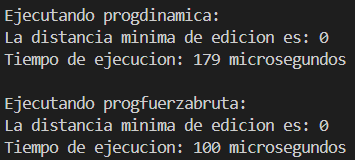
\includegraphics[width=0.6\textwidth]{./images/Resultados1.png}
  \caption{Resultados para el caso limite 1}
  \label{fig:imagen}
\end{figure}

2. Caso con cadenas repetidas:\\
\begin{figure}[ht]
  \centering
  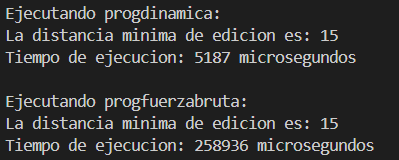
\includegraphics[width=0.6\textwidth]{./images/Resultados2.png}
  \caption{Resultados para el caso limite 2}
  \label{fig:imagen}
\end{figure}

3. Caso con cadenas simétricas:\\
\begin{figure}[ht]
  \centering
  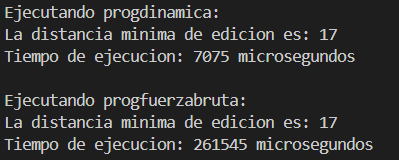
\includegraphics[width=0.6\textwidth]{./images/Resultados3.png}
  \caption{Resultados para el caso limite 3}
  \label{fig:imagen}
\end{figure}
\newpage
4. Caso con cadenas asimétricas:\\
\begin{figure}[ht]
  \centering
  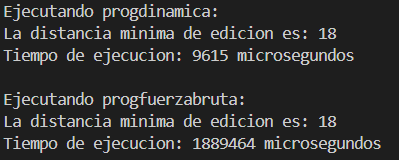
\includegraphics[width=0.6\textwidth]{./images/Resultados4.png}
  \caption{Resultados para el caso limite 4}
  \label{fig:imagen}
\end{figure}

5. Caso con matrices con valores iguales:\\
\begin{figure}[ht]
  \centering
  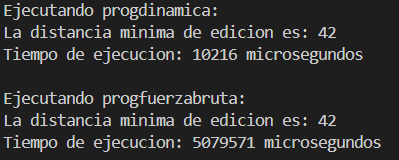
\includegraphics[width=0.6\textwidth]{./images/Resultados5.png}
  \caption{Resultados para el caso limite 5}
  \label{fig:imagen}
\end{figure}

6. Progresión respecto al aumento de caracteres:\\
\begin{figure}[ht]
  \centering
  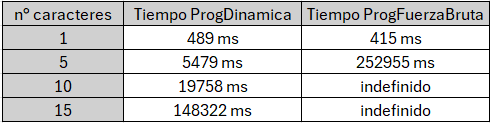
\includegraphics[width=0.6\textwidth]{./images/Resultados6.png}
  \caption{Resultados para la progresión con aumento de caracteres}
  \label{fig:imagen}
\end{figure}
\newpage
\subsection{Analisis de Resultados}

Es posible ver para la Fuerza Bruta que a medida que incrementa el número de caracteres en las cadenas de entrada, la cantidad de llamadas recursivas y los subproblemas a resolver aumenta drásticamente, lo que provoca una crecimiento exponencial del tiempo de ejecución. En experimentos prácticos, se observa que, para cadenas de longitud moderada, el tiempo de ejecución aumenta significativamente, y se vuelve inviable para cadenas más largas (por ejemplo, más de 10-12 caracteres). Esto se debe a que el número de subproblemas crece exponencialmente con el tamaño de las cadenas, lo que hace que el algoritmo sea muy lento.\\

La Programación Dinámica mejora considerablemente la eficiencia del algoritmo, ya que solo resuelve cada subproblema una vez. Este enfoque es significativamente más rápido en comparación con la fuerza bruta, especialmente cuando las cadenas tienen longitudes mayores. Los resultados experimentales muestran que incluso con cadenas de 100 o más caracteres, el algoritmo de Programación Dinámica es mucho más rápido y sigue siendo manejable en términos de tiempo de ejecución.\\

En el caso de cadenas simétricas, el algoritmo de Fuerza Bruta sigue siendo relativamente lento y peor que el de Programación Dinámica, ya que evalúa todas las combinaciones posibles de operaciones. Sin embargo, debido a la regularidad de la estructura de las cadenas, el número de subproblemas realmente distintos a resolver puede ser menor, lo que reduce parcialmente el tiempo de ejecución. Por otro lado, en el caso de cadenas asimétricas, la Fuerza Bruta se ve seriamente afectada. Debido a la falta de regularidad en la estructura de las cadenas, el número de subproblemas a resolver crece de manera exponencial.\\
